%& /home/radam/.config/TikzEdtWForms/TikzEdtWForms/0.2.1.0/temp_header
\begin{document}
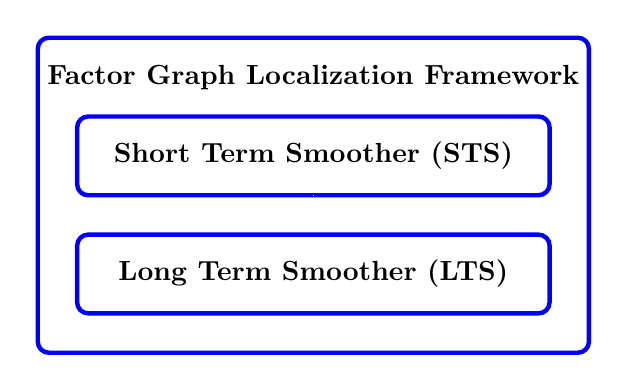
\begin{tikzpicture}

\draw [ultra thick, rounded corners, blue] (-2,4) rectangle (5,0);
\draw [ultra thick, rounded corners, blue] (-1.5,1.5) rectangle (4.5,0.5);
\draw [ultra thick, rounded corners, blue] (-1.5,3) rectangle (4.5,2);

\node [text centered,font=\bf] at (1.5,3.5) {Factor Graph Localization Framework};
\node [text centered,font=\bf] at (1.5,2.5) {Short Term Smoother (STS)};
\node [text centered,font=\bf] at (1.5,1) {Long Term Smoother (LTS)};


\usetikzlibrary{calc}
\pgftransformreset
\node[inner sep=0pt,outer sep=0pt,minimum size=0pt,line width=0pt,text width=0pt,text height=0pt] at (current bounding box) {};
%add border to avoid cropping by pdflibnet
\foreach \border in {0.1}
  \useasboundingbox (current bounding box.south west)+(-\border,-\border) rectangle (current bounding box.north east)+(\border,\border);
\newwrite\metadatafile
\immediate\openout\metadatafile=\jobname_BB.txt
\path
  let
    \p1=(current bounding box.south west),
    \p2=(current bounding box.north east)
  in
  node[inner sep=0pt,outer sep=0pt,minimum size=0pt,line width=0pt,text width=0pt,text height=0pt,draw=white] at (current bounding box) {
\immediate\write\metadatafile{\p1,\p2}
};
\immediate\closeout\metadatafile
\end{tikzpicture}

\end{document}
